\section{Task 1.1}
\begin{figure}[h]
  \centering
  \begin{subfigure}[t]{0.3\textwidth}
    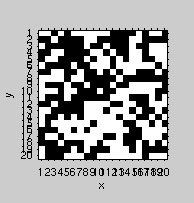
\includegraphics[width=\textwidth]{img/1_1_before.png}
    \caption{The randomly generated image.}
    \label{fig:1_1_before}
  \end{subfigure}%
  ~
  \begin{subfigure}[t]{0.3\textwidth}
    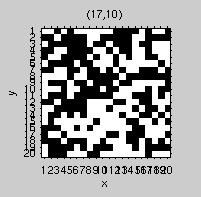
\includegraphics[width=\textwidth]{img/1_1_after.png}
    \caption{The randomly generated image with a blackened pixel as well as the
      coordinates.}
    \label{fig:1_1_after}
  \end{subfigure}
\end{figure}

This task was solved by generating a $20\times 20$ matrix of ones and
zeros. Then using ginput to retrieve the coordinates for a click and setting
that pixel to value $0$. Source code is in the appendix.
